\chapter{带电粒子、场变换与相对论性波}

上次我们开始追问：一旦引入相对性原理，带电粒子在电场和磁场中如何运动。熟悉的洛伦兹力定律已经给出了线索：其磁力项依赖于粒子的速度，因此不同的观测者不可能分别就什么是电场、什么是磁场达成一致。我们的任务是重新表述这一定律，使得每个惯性观测者都使用同一个方程，尽管场和粒子速度会随参考系而改变。

除非另有说明，我们采用\(c=1\)的单位制，度规符号差为\((-,-,-,+)\)。时空分量的排列顺序是三个空间分量在前：
\begin{equation}
  \mu=(1,2,3,0)=(x,y,z,t).
\end{equation}
拉丁字母指标\(m,n\)只取三个空间方向。

\section{牛顿力定律中幸存下来的部分}

在牛顿力学中，
\begin{equation}
  \boldsymbol F=m\boldsymbol a
\end{equation}
在每个惯性系中都具有相同的形式，因为伽利略观测者对加速度的看法一致。他们也为粒子赋予相同的质量和力。一旦运动学发生改变，就没有理由期望力与普通加速度之间的这一特定关系保持不变。

电磁学和引力已经警告我们，相对论性的推广不必彼此相似。库仑定律和牛顿万有引力定律都是平方反比定律，但引力若不经过时空几何的更深层改变，就无法自然地纳入狭义相对论。电磁学则可以。事实上，磁性本身就是一种相对论效应：当恢复\(c\)的因子时，磁力带有速度除以\(c\)的因子，并在形式极限\(c\to\infty\)下消失。

牛顿定律中持久的部分是：力是动量的变化率。对于恒定的静止质量，
\begin{equation}
  \boldsymbol F
  =m\frac{d\boldsymbol v}{dt}
  =\frac{d}{dt}(m\boldsymbol v)
  =\frac{d\boldsymbol p}{dt}.
\end{equation}
相对论将改变动量与速度之间的关系，但会保留这种组织方程的方式。

\begin{figure}[H]
\centering
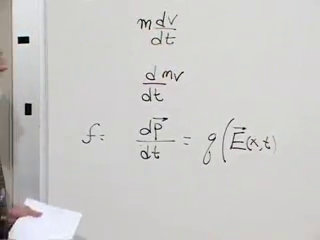
\includegraphics[width=0.64\textwidth]{lecture_07_figure_01.png}
\caption{当洛伦兹定律的电场部分被写在黑板上时，力被改写为\(d\boldsymbol p/dt\)。}
\lectureframe{00:08:20}
\end{figure}

在\(c=1\)的单位制下，前相对论性的洛伦兹力定律为
\begin{equation}
  \frac{d\boldsymbol p}{dt}
  =q\bigl(\boldsymbol E+\boldsymbol v\times\boldsymbol B\bigr).
  \label{eq:lorentz-three}
\end{equation}
两个场都可能依赖于位置和时间。非相对论极限现在是\(v\ll 1\)的极限，而不是数值常数\(c=1\)以某种方式发生改变的极限。\eqref{eq:lorentz-three}中的电场项已经是一个普通的矢量。为了以能够带入时空的形式理解磁力项，我们必须重新审视叉积。

\section{作为反对称张量的叉积}

取两个三维矢量\(\boldsymbol A\)和\(\boldsymbol B\)。它们的外积
\begin{equation}
  T_{mn}=A_mB_n
\end{equation}
是一个具有九个分量的二阶张量。它一般没有对称性。反对称化后得到
\begin{equation}
  K_{mn}=A_mB_n-A_nB_m,
  \qquad K_{mn}=-K_{nm}.
  \label{eq:antisym-product}
\end{equation}
其对角元为零，而对角线以下的每个元素都由其上方对应的元素确定。因此一个\(3\times3\)反对称张量只有三个独立分量。

这个计数具有启发性，但本身并不充分。三个量并不会自动像矢量那样变换。然而在三维中，\eqref{eq:antisym-product}的三个独立元素可以与叉积
\(\boldsymbol C=\boldsymbol A\times\boldsymbol B\)的分量等同起来。黑板首先将\(C_2\)临时放在右上位置：

\begin{figure}[H]
\centering
\includegraphics[width=0.75\textwidth]{lecture_07_figure_02.png}
\caption{反对称乘积，同时其三个独立元素正被与\(\boldsymbol C\)的分量进行匹配。右上角的标记在这里仍然是暂定的。}
\lectureframe{00:17:33}
\end{figure}

循环\(1\to2\to3\to1\)给出分量公式
\begin{align}
  C_3 &= A_1B_2-A_2B_1, \\
  C_1 &= A_2B_3-A_3B_2, \\
  C_2 &= A_3B_1-A_1B_3.
  \label{eq:cross-components}
\end{align}
最后一行表明右上角的元素是\(-C_2\)，而不是\(C_2\)。这一修正本身就是论证的一部分，而不是应当隐藏的细节。

\begin{figure}[H]
\centering
\includegraphics[width=0.62\textwidth]{lecture_07_figure_03.png}
\caption{完整的循环分量恒等式，它们确定了反对称阵列中临时符号。}
\lectureframe{00:21:54}
\end{figure}

由此得到的矩阵是
\begin{equation}
  K_{mn}=
  \begin{pmatrix}
    0 & C_3 & -C_2 \\
    -C_3 & 0 & C_1 \\
    C_2 & -C_1 & 0
  \end{pmatrix}.
  \label{eq:cross-matrix}
\end{equation}

这一记号背后有一个有用的几何图像。指标为\(1,2\)的分量自然属于\(xy\)平面，并被等同于沿垂直的\(z\)轴方向的矢量分量。人们可以用一个平面或用垂直于该平面的箭头来描述同一个有向对象。箭头的描述是三维所特有的；在更高维中，反对称二阶张量仍然存在，但其分量数目不再与矢量相同。因此，叉积得以推广的形式是张量，而不是垂直箭头。

等价地，选定一个定向之后，
\begin{equation}
  C_k=\frac12\epsilon_{kmn}K_{mn}.
\end{equation}
需要选定一个定向，这正是右手定则以及极矢量与轴矢量之间熟悉区别的来源。
\editorialnote{Levi--Civita 公式与轴矢量术语，是讲稿中明确展开的平面与法向几何的标准记号。}

\section{张量形式的磁场}

同样的对偶描述也适用于磁场。我们将其反对称空间张量定义为
\begin{equation}
  B_{mn}=
  \begin{pmatrix}
    0 & -B_3 & B_2 \\
    B_3 & 0 & -B_1 \\
    -B_2 & B_1 & 0
  \end{pmatrix}.
  \label{eq:magnetic-tensor}
\end{equation}
相对于 \eqref{eq:cross-matrix} 多出的整体符号是一个约定。
一旦选定，就必须一致地使用；改变全部三个矢量分量的符号，将以相反的定向约定描述同一个张量到矢量的等同。

\begin{figure}[H]
\centering
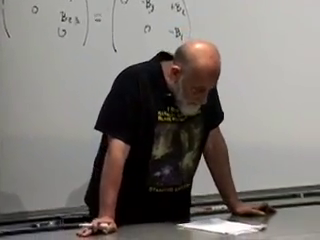
\includegraphics[width=0.72\textwidth]{lecture_07_figure_04.png}
\caption{磁场既写成反对称空间阵列，也用它三个矢量分量表示。}
\lectureframe{00:24:40}
\end{figure}

现在取叉积的第三个分量：
\begin{align}
  (\boldsymbol v\times\boldsymbol B)_3
  &=v_1B_2-v_2B_1 \\
  &=v_1B_{13}+v_2B_{23}+v_3B_{33}.
\end{align}
最后一项可以加上，因为 \(B_{33}=0\)。对自由分量进行轮换，得到紧凑规则
\begin{equation}
  (\boldsymbol v\times\boldsymbol B)_m=v_nB_{nm},
  \label{eq:cross-contraction}
\end{equation}
其中重复指标 \(n\) 被求和。因此磁力为
\begin{equation}
  F_m^{(B)}=qv_nB_{nm}.
\end{equation}

\begin{figure}[H]
\centering
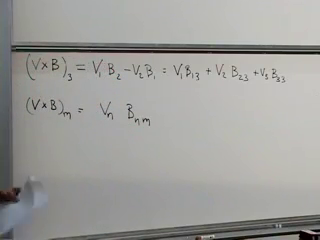
\includegraphics[width=0.78\textwidth]{lecture_07_figure_05.png}
\caption{\(\boldsymbol v\times\boldsymbol B\) 的第三个分量及其作为与 \(B_{nm}\) 缩并的一般表达式。}
\lectureframe{00:28:30}
\end{figure}

\begin{classroomqa}
\audiencequestion{自由指标 \(m\) 是否标记力的一个单独的磁分量？}
\lecturerresponse{不是。它标记的是正在计算的力的任意一个空间分量。为当前论证起见，电场已被简单地设为零，而这里的每个指标都只遍历三个空间方向。}
\end{classroomqa}

张量记号使磁场的无功性质几乎自动成立。对速率的平方求导：
\begin{align}
  \frac{d}{dt}(v_mv_m)
  &=2\dot v_m v_m \\
  &\propto 2(\boldsymbol v\times\boldsymbol B)_m v_m \\
  &=2v_nB_{nm}v_m.
  \label{eq:speed-derivative}
\end{align}
含 \(m=n\) 的项消失，因为 \(B_{nm}\) 的对角线为零。每个非对角项都有一个将 \(m\) 与 \(n\) 互换的配对项；二者相消，因为 \(v_nv_m\) 对称而 \(B_{nm}\) 反对称。
因此
\begin{equation}
  \frac{d}{dt}(v_mv_m)=0.
\end{equation}
纯磁力使轨迹弯曲，而不改变其速率或动能。

\begin{figure}[H]
\centering
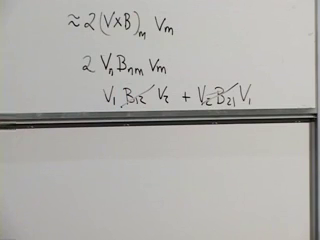
\includegraphics[width=0.68\textwidth]{lecture_07_figure_06.png}
\caption{\(v_nB_{nm}v_m\) 中的配对项相消，因为磁张量在交换其指标时改变符号。}
\lectureframe{00:35:40}
\end{figure}

这个证明有意比说叉积垂直于其第一个因子更为繁复。后一说法是三维矢量表示所特有的。对称对与反对称张量的缩并，才是将在四维中继续成立的论证。

\begin{classroomqa}
\audiencequestion{磁场是否必须与时间无关，速率才能保持恒定？}
\lecturerresponse{上述代数从未对场求导，也不要求 \(\partial_t\boldsymbol B=0\)。单独的磁项仍然不做功。然而在电动力学中，变化的磁场会产生电场，而该电场可以改变粒子的速率。}
\end{classroomqa}

\section{为什么电场与磁场必须混合}

在任何四维计算之前，就可以看出 \(\boldsymbol E\) 与 \(\boldsymbol B\) 的混合。考虑慢速运动，使得关于加速度的普通牛顿陈述足够。设磁场沿 \(y\) 轴，并设带电粒子沿 \(x\) 轴运动。磁力沿 \(z\) 轴：
\begin{equation}
  \boldsymbol F=q\boldsymbol v\times\boldsymbol B.
\end{equation}

\begin{figure}[H]
\centering
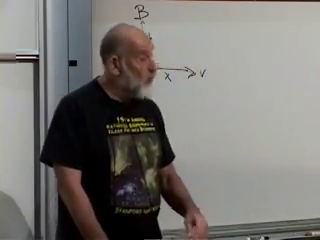
\includegraphics[width=0.62\textwidth]{lecture_07_figure_07.png}
\caption{粒子穿过磁场运动的板书草图；这三个方向用于比较实验室描述与共动描述。}
\lectureframe{00:42:20}
\end{figure}

可以不用教室的透视重新绘制该几何：
\begin{figure}[H]
\centering
\begin{tikzpicture}[scale=1.05,>=Stealth]
  \draw[->] (0,0) -- (3.8,0) node[right] {\(x\)};
  \draw[->] (0,0) -- (-1.9,2.4) node[above left] {\(y\)};
  \draw[->] (0,0) -- (0,3.1) node[above] {\(z\)};
  \draw[->,very thick] (0,0) -- (2.7,0)
    node[midway,below] {\(\boldsymbol v\)};
  \draw[->,very thick] (0,0) -- (-1.35,1.7)
    node[midway,above left] {\(\boldsymbol B\)};
  \draw[->,very thick] (0,0) -- (0,2.35)
    node[midway,right] {\(\boldsymbol F,\ \boldsymbol E'\)};
\end{tikzpicture}
\caption{在实验室中，沿 \(z\) 方向的力是磁力；在瞬时共动系中，同一个力必须是电力。}
\end{figure}

现在引入一个在该瞬间与粒子一起运动的观察者。粒子在新参考系中的速度为零，因此磁项 \(q\boldsymbol v'\times\boldsymbol B'\) 消失。然而在慢速运动极限下，两个观察者都必须同意粒子具有沿 \(z\) 的加速度。如果洛伦兹力定律在两个参考系中具有相同形式，那么共动观察者必须把该力归因于沿 \(z\) 的电场 \(\boldsymbol E'\)。因此，在实验室中纯为磁性的场，在运动参考系中并非纯为磁性。

这就是寻求一个其分量同时包含两种场的对象的物理原因。参考系的改变不只是让\(\boldsymbol E\)和\(\boldsymbol B\)各自的三个分量分别发生旋转；它还会混合这两组分量。

\section{电磁场张量}

电场和磁场合起来共有六个分量。一个四维反对称张量同样有六个独立分量，因为
\begin{equation}
  \frac{4(4-1)}{2}=6.
\end{equation}
这并不意味着反对称张量真的是人们所能构造出的唯一一种包含六个量的集合：六个标量，或者一个矢量加两个标量，也同样包含六个数。它是其分量能够以所需方式混合的自然几何客体。

为使板书约定明确，我们按空间分量在前的顺序\((1,2,3,0)\)写出逆变张量：
\begin{equation}
  F^{\mu\nu}=
  \begin{pmatrix}
    0 & -B_3 & B_2 & E_1 \\
    B_3 & 0 & -B_1 & E_2 \\
    -B_2 & B_1 & 0 & E_3 \\
    -E_1 & -E_2 & -E_3 & 0
  \end{pmatrix}.
  \label{eq:l07-field-tensor}
\end{equation}
左上角的\(3\times3\)分块正是磁张量\eqref{eq:magnetic-tensor}；带一个空间指标和一个时间指标的分量包含电场。反对称性给出了其余的元素。

\begin{figure}[H]
\centering
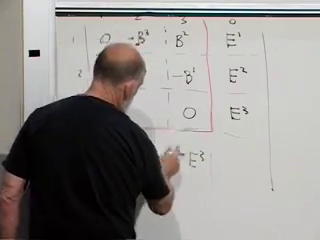
\includegraphics[width=0.72\textwidth]{lecture_07_figure_08.png}
\caption{磁性的空间分块与电性的时间-空间列被组装成四维场张量。}
\lectureframe{00:46:35}
\end{figure}

\begin{classroomqa}
\audiencequestion{这些场分量什么时候应当带上指标而不是下指标？}
\lecturerresponse{仅就三个空间标号而言，在辨认熟悉的麦克斯韦--法拉第场时，板书有时会略去这一区别。在协变计算中则必须恢复这一区别：在所选的度规约定下，升高或降低一个空间指标会改变一个符号。}
\end{classroomqa}

不变的不是板书上某种特定的符号排列，而是反对称的时空张量，连同自洽的度规与指标约定。记号\(F\)可能让人联想到法拉第，尽管本讲并不自信地主张这一历史归属。爱因斯坦在1905年给出了电场和磁场分量的变换；紧凑的四维张量语言则随着后来与闵可夫斯基相联系的时空表述而出现。

\section{四维速度与四维力}

方程中粒子一侧也必须协变化。固有时\(\tau\)是不变量，因此用它对位置四维矢量求导得到另一个四维矢量：
\begin{equation}
  u^\mu=\frac{dx^\mu}{d\tau}
  =\gamma(v_x,v_y,v_z,1),
  \qquad
  \gamma=\frac{1}{\sqrt{1-v^2}}.
  \label{eq:four-velocity}
\end{equation}
最后一个分量由\(dt/d\tau=\gamma\)得出。四维动量为
\begin{equation}
  p^\mu=mu^\mu,
\end{equation}
其空间部分就是相对论动量
\(\boldsymbol p=m\gamma\boldsymbol v\)。

\begin{figure}[H]
\centering
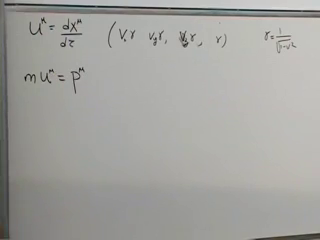
\includegraphics[width=0.75\textwidth]{lecture_07_figure_09.png}
\caption{四维速度、其分量、洛伦兹因子以及四维动量。}
\lectureframe{00:50:30}
\end{figure}

因为\(p^\mu\)是四维矢量而\(\tau\)是标量，自然的相对论性左端为
\begin{equation}
  f^\mu\equiv\frac{dp^\mu}{d\tau}.
  \label{eq:four-force-def}
\end{equation}
四维力不能任意选取。四维速度具有固定的模，
\begin{equation}
  u_\mu u^\mu=1.
\end{equation}
沿世界线求导给出
\begin{align}
  0
  &=\frac{d}{d\tau}(u_\mu u^\mu) \\
  &=\frac{du_\mu}{d\tau}u^\mu
    +u_\mu\frac{du^\mu}{d\tau} \\
  &=2u_\mu\frac{du^\mu}{d\tau}.
\end{align}
对于恒定质量，这意味着
\begin{equation}
  f^\mu u_\mu=0.
  \label{eq:force-orthogonal}
\end{equation}
因此四维力与四维速度闵可夫斯基正交。这是由\(u^\mu\)的归一化得出的纯运动学约束，而不是电磁学特有的性质。

\begin{figure}[H]
\centering
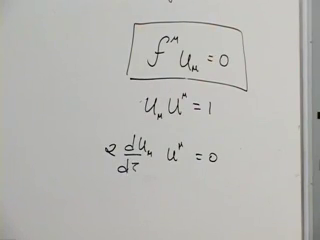
\includegraphics[width=0.64\textwidth]{lecture_07_figure_10.png}
\caption{四维速度的单位模以及由此得到的四维力与四维速度的正交性。}
\lectureframe{00:56:50}
\end{figure}

三维磁性的计算已经提供了满足\eqref{eq:force-orthogonal}的技巧。将一个反对称张量与速度的一份拷贝缩并：
\begin{equation}
  \boxed{
  \frac{dp^\mu}{d\tau}=qF^{\mu\nu}u_\nu.}
  \label{eq:covariant-lorentz}
\end{equation}
确实，
\begin{equation}
  f^\mu u_\mu
  =qF^{\mu\nu}u_\nu u_\mu=0,
\end{equation}
因为\(F^{\mu\nu}\)是反对称的而\(u_\nu u_\mu\)是对称的。这并不是唯一可能的相对论性力律，但它是对电磁场和速度都线性的最简单的一个。

\begin{figure}[H]
\centering
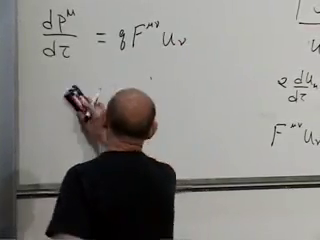
\includegraphics[width=0.72\textwidth]{lecture_07_figure_11.png}
\caption{左边是协变洛伦兹力方程，右边是它与第二个四维速度的缩并为零。}
\lectureframe{01:00:00}
\end{figure}

\section{恢复通常的洛伦兹力}

一个看似协变的方程仍必须重现已知的力律。按照开头所述的度规约定，
\begin{equation}
  u_\mu=\gamma(-v_x,-v_y,-v_z,1).
\end{equation}
对于\(x\)分量，\eqref{eq:l07-field-tensor}和\eqref{eq:covariant-lorentz}给出
\begin{align}
  \frac{dp^1}{d\tau}
  &=q\bigl(F^{12}u_2+F^{13}u_3+F^{10}u_0\bigr) \\
  &=q\gamma\bigl(B_3v_y-B_2v_z+E_1\bigr) \\
  &=q\gamma\bigl[\boldsymbol E+\boldsymbol v\times
    \boldsymbol B\bigr]_x.
  \label{eq:x-force}
\end{align}
其余空间分量可通过循环置换指标得到。

\begin{classroomqa}
\audiencequestion{分量展开中的\(qE_x\)项在哪里？}
\lecturerresponse{它就是\(qF^{10}u_0\)项。带一个空间指标和一个时间指标的场张量分量是电场分量，而\(u_0=\gamma\)。}
\end{classroomqa}

右端的因子\(\gamma\)并不是额外的力。由于
\begin{equation}
  \frac{dp^i}{d\tau}=\frac{dt}{d\tau}\frac{dp^i}{dt}
  =\gamma\frac{dp^i}{dt},
\end{equation}
它从\eqref{eq:x-force}的两端消去。因此精确的空间方程仍然是
\begin{equation}
  \frac{d\boldsymbol p}{dt}
  =q\bigl(\boldsymbol E+\boldsymbol v\times\boldsymbol B\bigr),
  \qquad
  \boldsymbol p=m\gamma\boldsymbol v.
  \label{eq:exact-three-force}
\end{equation}
熟悉的形式保留了下来，但相对论性隐藏在动量之中。

\begin{figure}[H]
\centering
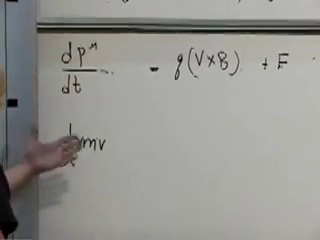
\includegraphics[width=0.75\textwidth]{lecture_07_figure_12.png}
\caption{去掉共同的固有时因子后，就恢复了三维洛伦兹定律；动量仍保留其\(\gamma\)因子。}
\lectureframe{01:06:30}
\end{figure}

时间分量承载着相应的能量陈述，
\begin{equation}
  \frac{dp^0}{dt}=q\boldsymbol E\cdot\boldsymbol v,
\end{equation}
因此磁场不做功，而电场可以改变粒子的能量。
\editorialnote{时间分量的检验是讲座中空间计算的直接对应部分；引入它是为了在四维记号中揭示同样的不做功性质。}

\begin{classroomqa}
\audiencequestion{这个推导是数学还是物理？}
\lecturerresponse{两者都是。张量代数提供了紧凑的形式，但实质性的物理内容是通过所有惯性系服从相同定律这一原理，以及运动方程为二阶这一假设进入的。二阶定律由位置和速度预测未来；三阶定律则需要把加速度作为额外的初始数据。是实验，而不是记号，告诉我们自然界使用哪一种定律。}
\end{classroomqa}

\section{场如何变换}

方程\eqref{eq:covariant-lorentz}在每个参考系中都具有相同的形式，因为两边都是四维矢量。场张量本身的变换则对每个指标各用一个洛伦兹矩阵：
\begin{equation}
  F'^{\mu\nu}
  =\Lambda^\mu{}_{\rho}\Lambda^\nu{}_{\sigma}F^{\rho\sigma}.
  \label{eq:tensor-transform}
\end{equation}
黑板上通过先变换一个简单的乘积\(A^\mu B^\nu\)来推导这条规则。一旦知道了矢量乘积的规则，线性性就给出了任意二阶张量的规则。

对于沿\(1\)轴的推动，坐标的变换为
\begin{align}
  x'^1&=\gamma(x^1-vx^0), &
  x'^0&=\gamma(x^0-vx^1), \\
  x'^2&=x^2, & x'^3&=x^3.
\end{align}
对两个张量指标分别施加同样的变换。对于平行于推动方向的分量，黑板从一个乘积开始：
\begin{align}
  (A'^0B'^1)
  =\gamma^2\bigl(
     A^0B^1-vA^0B^0-vA^1B^1+v^2A^1B^0
   \bigr).
\end{align}
把每个乘积替换为相应的张量分量，然后利用反对称性\(F^{00}=F^{11}=0\)和\(F^{10}=-F^{01}\)，得到
\begin{equation}
  F'^{01}
  =\gamma^2(1-v^2)F^{01}
  =F^{01}.
\end{equation}
因此平行于运动的电场分量不变。平行的磁场分量行为类似。

横向分量则不同。按照黑板上使用的带撇参考系和符号约定，
\begin{align}
  F'^{02}
  &=\gamma\bigl(F^{02}-vF^{12}\bigr), \\
  E'_2
  &=\gamma(E_2+vB_3).
  \label{eq:e-transform}
\end{align}
一个横向电场分量获得了一部分磁场分量。其余的变换定律由同样的双指标规则得出，留作讲座的练习。

\begin{figure}[H]
\centering
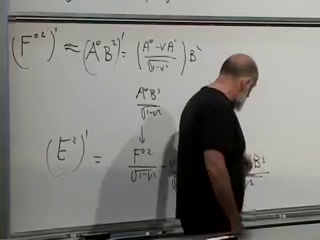
\includegraphics[width=0.76\textwidth]{lecture_07_figure_13.png}
\caption{在\(E'_2\)分量处，横向张量变换被看到包含一个正比于\(vB_3\)的项。}
\lectureframe{01:23:40}
\end{figure}

\eqref{eq:e-transform}中的符号取决于哪个参考系被声明为以\(+v\)运动，也取决于指标和度规约定。其不变内容则不取决于这些：横向电场和磁场分量相互混合，而变换之后协变力方程仍然成立。

\begin{classroomqa}
\audiencequestion{对于导线中的电流，能否以某个速度运动从而使磁场消失？}
\lecturerresponse{随传导电子一起运动是不够的，因为这样一来正晶格电荷就在新参考系中运动了。因此，一条中性的载流导线比单个运动的电荷团更微妙。纯磁场不能被完全变换掉。如果电场和磁场同时存在，它们的变换部分在特殊情况下可以相消；对于单个匀速运动的电荷，电荷的静止系就是使其磁场消失的简单参考系。}
\end{classroomqa}

精确的不变判据使用
\begin{equation}
  \boldsymbol B^2-\boldsymbol E^2,
  \qquad
  \boldsymbol E\cdot\boldsymbol B.
\end{equation}
只有当电场占主导且\(\boldsymbol E\cdot\boldsymbol B=0\)时，才可能存在满足\(\boldsymbol B'=0\)的参考系；在一个参考系中为纯磁场的场是磁场占主导的，不能满足该条件。
\editorialnote{这些不变判据精确地陈述了课堂讨论中得到的限定条件；它们的推导被推迟。}

\begin{classroomqa}
\audiencequestion{电标势和磁矢势构成一个四维矢量吗？}
\lecturerresponse{是的。在依赖于约定的符号下，它们组合成四维势\(A^\mu\)。麦克斯韦方程组将系统地使用这个对象。}
\end{classroomqa}

\section{场的导数}

现在我们离开单个粒子的轨迹，考虑遍布时空的场。设
\begin{equation}
  \phi=\phi(x^1,x^2,x^3,x^0)
\end{equation}
为一个标量场。它的四个导数构成一个四维矢量的协变分量：
\begin{equation}
  \partial_\mu\phi
  \equiv\frac{\partial\phi}{\partial x^\mu}
  =\left(
    \frac{\partial\phi}{\partial x},
    \frac{\partial\phi}{\partial y},
    \frac{\partial\phi}{\partial z},
    \frac{\partial\phi}{\partial t}
  \right).
\end{equation}
对洛伦兹坐标变换应用链式法则，就证明了这条协变变换定律。升高指标会反转空间符号，但时间符号保持不变：
\begin{equation}
  \partial^\mu\phi
  =\left(
    -\frac{\partial\phi}{\partial x},
    -\frac{\partial\phi}{\partial y},
    -\frac{\partial\phi}{\partial z},
    \frac{\partial\phi}{\partial t}
  \right).
\end{equation}

每一次微分都会贡献一个下指标。因此，\(\partial_\nu V^\mu\) 是一个具有一个上指标和一个下指标的二阶张量，而对张量求导会产生一个额外多出一个下指标的对象。这就是在不选择任何优先惯性系的情况下写出场方程所需的基本规则。

\section{不变标量波动方程}

最简单的波动方程包含两个导数。如果该方程要在每个惯性系中都具有相同形式，其左侧就应当是一个标量。对导数指标进行缩并，得到唯一最简单的选择：
\begin{equation}
  \boxed{\partial^\mu\partial_\mu\phi=0.}
  \label{eq:wave-covariant}
\end{equation}
在当前号差下写出其分量，
\begin{equation}
  \frac{\partial^2\phi}{\partial t^2}
  -\frac{\partial^2\phi}{\partial x^2}
  -\frac{\partial^2\phi}{\partial y^2}
  -\frac{\partial^2\phi}{\partial z^2}=0.
  \label{eq:wave-components}
\end{equation}
\eqref{eq:wave-covariant} 中的缩并使洛伦兹不变性显而易见；方程 \eqref{eq:wave-components} 则是同一陈述按分量逐项写出的形式。

\begin{figure}[H]
\centering
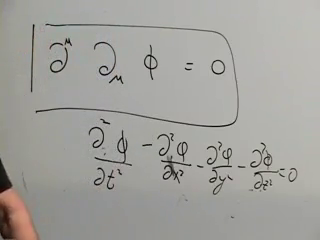
\includegraphics[width=0.75\textwidth]{lecture_07_figure_14.png}
\caption{标量波动方程的缩并导数形式及其时间减空间的分量展开。}
\lectureframe{01:39:40}
\end{figure}

\begin{classroomqa}
\audiencequestion{波动方程的右侧必须为零吗？}
\lecturerresponse{不。它可以是任何与问题相容的标量。一个常数乘以 \(\phi\)，或者一个非线性标量函数，例如与 \(\phi^2\) 成正比的函数，仍然保持协变性。取零则给出最简单的自由波动方程。}
\end{classroomqa}

这个标量示例的意义在于作准备。麦克斯韦方程组以更复杂的方式混合电场和磁场，但它们同样可以被写成使其洛伦兹不变性从指标结构中显而易见的形式。这就是我们下次要回到的问题。